\documentclass[11pt, a4paper]{article}

% Department template: Presentation_Report_Guideline_LaTeX_Source, case 1 (research project).
% Every number in this report is read from a result file named beside it; see docs/reports/phase2_latex/README.md.

\usepackage[utf8]{inputenc}
\usepackage[T1]{fontenc}
\usepackage{mathptmx}
\usepackage{amsmath,amssymb}
\usepackage{graphicx}
\usepackage[margin=0.8in]{geometry}
\usepackage{xcolor}
\usepackage{titlesec}
\usepackage{enumitem}
\usepackage{float}
\usepackage{booktabs}
\usepackage{multirow}
\usepackage{array}
\usepackage{tikz}
\usetikzlibrary{positioning, arrows.meta}
\usepackage[hidelinks]{hyperref}

\definecolor{amritaMaroon}{HTML}{A4123F}
\titlespacing*{\section}{0pt}{12pt}{4pt}
\titlespacing*{\subsection}{0pt}{8pt}{3pt}
\titleformat{\section}{\large\bfseries\color{amritaMaroon}}{\thesection}{0.8em}{}
\titleformat{\subsection}{\normalsize\bfseries\color{amritaMaroon}}{\thesubsection}{0.6em}{}
\pagestyle{plain}

\begin{document}

\noindent
\begin{minipage}{\textwidth}
    \centering
    {\Large \textbf{\textcolor{amritaMaroon}{
    AMRITA VISHWA VIDYAPEETHAM \\
    SCHOOL OF COMPUTING \\
    DEPARTMENT OF COMPUTER SCIENCE AND ENGINEERING \\
    }}}
    \vspace{0.2cm}
    {\large \textbf{MOF Graphs and Crystal Morphology: Crystal Shapes of Metal--Organic Frameworks from the Unit Cell}} \\[0.1cm]
    \textbf{23CSE498 -- Project Phase II (External Review)} \quad | \quad \textbf{Team Number: G070} \\
    13 November 2026
\end{minipage}

\vspace{0.3cm}
\hrule
\vspace{0.3cm}

\noindent
\begin{center}
    \renewcommand{\arraystretch}{1.4}
    \setlength{\tabcolsep}{6pt}
    \begin{tabular}{|l|p{4.6cm}|p{4.3cm}|p{3.0cm}|}
        \hline
        \multicolumn{2}{|c|}{\textbf{Team Members}} & \textbf{Project Guide} & \textbf{Project Type} \\
        \hline
        \small CB.SC.U4CSE23134 & \small \raggedright Pasupuleti Meena Radha Krishna &
        \multirow{5}{=}{\raggedright \small \textbf{Dr. T. Ramraj} \newline \textit{Assistant Professor (Sl. Gd.), \newline Dept. of CSE}} &
        \multirow{5}{=}{\raggedright \small \textbf{Type 1} \newline Research-Based Project} \\ \cline{1-2}
        \small CB.SC.U4CSE23122 & \small Kshitij Varma Pinnamaraju & & \\ \cline{1-2}
        \small CB.SC.U4CSE23031 & \small Keerthi Sree Jonnakuti & & \\ \cline{1-2}
        \small CB.SC.U4CSE23141 & \small Rohith Abhinav Sai Komal Gullolla & & \\ \cline{1-2}
        \small CB.SC.U4CSE23029 & \small Isha Sri Prakash & & \\
        \hline
    \end{tabular}
\end{center}
\vspace{0.1cm}

\section{Abstract}
\noindent
A metal--organic framework (MOF) is used as a powder of small crystals, and the faces and size of those crystals affect how fast a gas enters them. After Panel Review~1 the panel asked whether a few crystal morphologies can be generated from the unit cell of an established MOF, mathematically and computationally. We answer in three steps. The space group decides which crystal faces may exist and gives a family of possible shapes (16 propositions, each proved and checked numerically). A growth model selects a member of the family: the Bravais--Friedel--Donnay--Harker (BFDH) rule for any lattice, and a Wulff construction from unrelaxed surface energies that are, in effect, a count of the bonds each plane cuts. The predictions are scored against 134 laboratory records from 35 papers on 12 MOFs. For crystals grown without additives the dominant face is predicted correctly for 4 of 5 MOFs, as often as the most common laboratory answer for each MOF, without using laboratory data; with additives no model is reliable. For eight MOFs we also compute how far each face's energy must fall to change the shape and, for each shape, the fraction of each face open to CO$_2$ and N$_2$ and the diffusion length $V/A$. Everything runs from a CIF in seconds, in two independent implementations (Python and a browser engine) that agree. An earlier connectivity descriptor (Part~I) was tested and withdrawn because it follows graph size.

\section{Problem Definition, Research Motivation \& Literature Review}

\subsection{Problem Statement \& Research Motivation}
\begin{itemize}[noitemsep, topsep=2pt]
    \item \textbf{Problem Statement:} Given the CIF (unit cell and atom positions) of an established MOF, generate the crystal morphologies it can take, decide which is favoured, and check the prediction against laboratory crystals.
    \item \textbf{Research Motivation:} A gas enters a crystal through its surface. The shape decides which faces form that surface and how much surface there is per volume, so two batches of one MOF can take up gas at different rates although their pores are identical. Knowing the possible shapes, and how hard each is to reach, tells a chemist what to try before weeks of synthesis.
    \item \textbf{Research Objectives:}
    \begin{enumerate}[noitemsep, topsep=2pt]
        \item Derive the allowed faces and the family of shapes of any MOF from its space group, with proofs.
        \item Select the favoured shape with a geometric (BFDH) and an energetic (Wulff) model, and score both against laboratory records with baselines that use the laboratory data.
        \item Connect shape to gas access with computed indicators, and state where the evidence stops.
    \end{enumerate}
\end{itemize}

\subsection{Literature Review \& Research Gap}
\begin{table}[H]
    \centering
    \footnotesize
    \renewcommand{\arraystretch}{1.2}
    \begin{tabular}{|p{2.8cm}|p{4.2cm}|p{4.2cm}|p{3.4cm}|}
        \hline
        \textbf{Author / Year} & \textbf{Core Methodology} & \textbf{Key Findings / Strengths} & \textbf{Limitations for MOFs} \\
        \hline
        Donnay \& Harker, 1937 \cite{donnay1937} & Growth rate $\propto 1/d_\text{eff}$, absences from the space group & Needs only lattice and symmetry & No energy, solvent or additive \\
        \hline
        Wulff; Miracle-Sol\'e, 2013 \cite{miracle2013} & Equilibrium shape from face energies & Exact construction & Needs reliable surface energies \\
        \hline
        Hartman--Perdok; Grimbergen et al., 1998 \cite{grimbergen1998} & Periodic bond chains, attachment energy & Links bonding to faces & Written for molecular and ionic crystals \\
        \hline
        Chen et al., 2020 \cite{chen2020} & Link counting and synthesis screening for one MOF family & One MOF, many shapes & One family; no general structure-only rule \\
        \hline
        Deng et al., 2023 \cite{deng2023} & CHGNet machine-learned potential & Fast energies for any crystal & Not validated for MOF surfaces \\
        \hline
    \end{tabular}
    \caption{Literature surveyed and the limitations that matter here.}
\end{table}
\noindent
\textbf{Research gap:} the methods exist separately, but no tool goes from a MOF's CIF to its allowed faces, its family of shapes, a structure-only prediction scored against many laboratory records, and the effect of shape on gas access, with each step checked.

\section{Proposed Methodology \& Solution Design}

\subsection{End-to-End Methodological Workflow}
\begin{figure}[H]
\centering
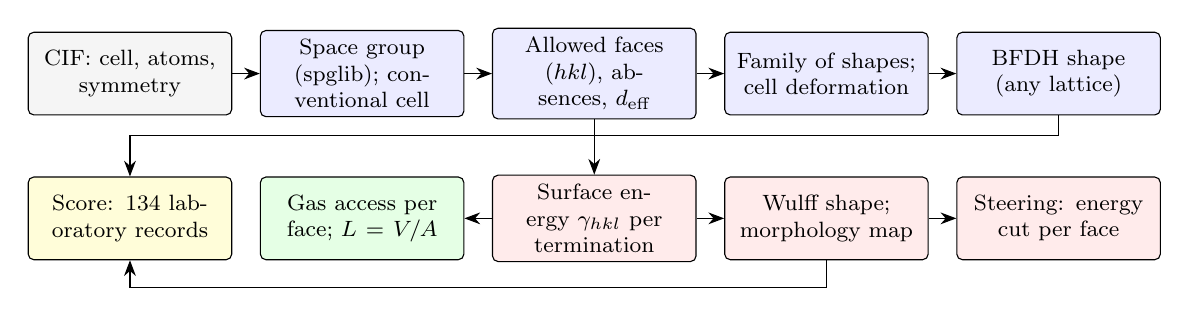
\begin{tikzpicture}[node distance=0.35cm and 0.35cm, every node/.style={font=\footnotesize, align=center},
  box/.style={draw, rounded corners=2pt, minimum height=1.05cm, text width=2.35cm, fill=#1}, box/.default=gray!8, >={Stealth[length=2mm]}]
\node[box] (cif) {CIF: cell, atoms, symmetry};
\node[box=blue!8, right=of cif] (sym) {Space group (spglib); conventional cell};
\node[box=blue!8, right=of sym] (faces) {Allowed faces $(hkl)$, absences, $d_\text{eff}$};
\node[box=blue!8, right=of faces] (fam) {Family of shapes; cell deformation};
\node[box=blue!8, right=of fam] (bfdh) {BFDH shape (any lattice)};
\node[box=red!8, below=0.7cm of faces] (gam) {Surface energy $\gamma_{hkl}$ per termination};
\node[box=red!8, right=of gam] (wulff) {Wulff shape; morphology map};
\node[box=red!8, right=of wulff] (steer) {Steering: energy cut per face};
\node[box=green!10, left=of gam] (acc) {Gas access per face; $L=V/A$};
\node[box=yellow!15, left=of acc] (lab) {Score: 134 laboratory records};
\draw[->] (cif) -- (sym); \draw[->] (sym) -- (faces); \draw[->] (faces) -- (fam); \draw[->] (fam) -- (bfdh);
\draw[->] (faces) -- (gam); \draw[->] (gam) -- (wulff); \draw[->] (wulff) -- (steer);
\draw[->] (gam) -- (acc); \draw[->] (bfdh.south) |- ++(0,-0.25) -| (lab.north); \draw[->] (wulff.south) |- ++(0,-0.35) -| (lab.south);
\end{tikzpicture}
\caption{Workflow. Blue: geometry from the unit cell. Red: energies and shapes. Green: gas access. Yellow: validation.}
\end{figure}

\subsection{Mathematical Formulation \& Algorithmic Design}
\begin{itemize}[noitemsep, topsep=2pt]
    \item \textbf{Allowed faces:} a reflection $(hkl)$ is absent when a symmetry operation $(R, \mathbf{t})$ has $\mathbf{h}R = \mathbf{h}$ and $\mathbf{h}\cdot\mathbf{t} \notin \mathbb{Z}$; the effective spacing is $d_\text{eff} = d_{hkl}/n$ with $n$ the smallest non-absent order.
    \item \textbf{BFDH:} face distance $\propto 1/d_\text{eff}$; the shape is $\{\mathbf{x} : \hat{\mathbf{n}}_{hkl}\cdot\mathbf{x} \le d_{\text{eff,max}}/d_\text{eff}\}$.
    \item \textbf{Surface energy:} $\gamma(s) = \tfrac12 (d/V)\sum_\text{pairs} \varepsilon_\text{pair}\, c_\text{pair}(s)$, the minimum over plane offsets $s$ giving the termination. Every cut bond costs 70~kcal/mol and UFF van der Waals terms \cite{rappe1992} add 2--7\%, so the face order is set by bonds cut per area.
    \item \textbf{Cubic morphology map:} the Wulff shape depends only on $x=\gamma_{110}/\gamma_{100}$ and $y=\gamma_{111}/\gamma_{100}$; cube for $y\ge\sqrt3,\ x\ge\sqrt2$; octahedron for $y\le 1/\sqrt3,\ x\ge\sqrt{3/2}\,y$; rhombic dodecahedron for $x\le1/\sqrt2,\ y\ge\sqrt{3/2}\,x$.
    \item \textbf{Gas access:} a point of a face is open when a probe of radius 1.65~\AA{} (CO$_2$) or 1.82~\AA{} (N$_2$) fits without overlap (Bondi radii); diffusion length $L = \Psi V^{1/3}/(36\pi)^{1/3} = V/A$.
    \item \textbf{Dataset:} 134 laboratory records (35 papers, 12 MOFs) with shape, faces, conditions and figure source; structures for 8 MOFs (two more with stand-ins).
    \item \textbf{Evaluation:} dominant face and habit (compact, rod, plate) against each record; baselines are the per-MOF laboratory majority with each paper held out, and the majority of the other MOFs with the whole MOF held out; Wilson intervals and a bootstrap over whole papers.
\end{itemize}

\section{Implementation Details}

\subsection{Implementation Environment \& Execution Setup}
\begin{itemize}[noitemsep, topsep=2pt]
    \item \textbf{Hardware:} ordinary CPU for every result in this report; CHGNet slab runs used a Google Colab GPU.
    \item \textbf{Software:} Python 3.11--3.13 (numpy, scipy, networkx, ase, spglib, matplotlib, pandas); JavaScript in the browser with three.js; jsdom tests under Node.js.
    \item \textbf{Repository:} \url{https://github.com/Radha-Krishna-19/fyp}; \newline website \url{https://radha-krishna-19.github.io/fyp/}.
\end{itemize}

\subsection{Module-Wise Implementation \& Integration Summary}
\begin{table}[H]
    \centering
    \footnotesize
    \renewcommand{\arraystretch}{1.2}
    \begin{tabular}{|p{3.3cm}|p{9.0cm}|c|}
        \hline
        \textbf{Module} & \textbf{Implemented details and files} & \textbf{Status} \\
        \hline
        Structure and symmetry & CIF reading, symmetry expansion, conventional cell (\texttt{mofmorph/structure.py}, \texttt{mof\_cif\_shape.js}) & Integrated \\
        \hline
        Faces and shapes & Absences, $d_\text{eff}$, BFDH, shape families, deformed cells, any lattice (\texttt{faces.py}, \texttt{deform.py}, \texttt{mof\_general\_shape.js}) & Integrated \\
        \hline
        Energies & Bond-count/UFF cleavage energies (\texttt{forcefield.py}); CHGNet slabs (\texttt{chgnet\_wulff/}, unvalidated) & Integrated \\
        \hline
        Benchmark, steering, access & \texttt{run\_benchmark\_mofs.py}, \texttt{run\_shape\_steering.py}, \texttt{run\_shape\_adsorption.py}, \texttt{run\_dataset\_shapes.py} & Integrated \\
        \hline
        Website and tests & 27 pages built from fragments; 15 jsdom suites (over 3\,400 checks) and the Python tests pass & Functional \\
        \hline
    \end{tabular}
    \caption{Module-wise implementation status.}
\end{table}
\noindent
Every script finds its inputs from its own location and writes a result file that names it. The Python and browser implementations were written separately and are compared number by number in the tests; a disagreement means one of them is wrong.

\section{Verification, Experimental Results \& Demonstration}

\subsection{Quantitative Evaluation \& Baseline Comparison}
\begin{table}[H]
    \centering
    \footnotesize
    \renewcommand{\arraystretch}{1.2}
    \begin{tabular}{|p{5.4cm}|c|c|c|}
        \hline
        \textbf{Model (dominant face)} & \textbf{No additive (32)} & \textbf{With additive (44)} & \textbf{All (76)} \\
        \hline
        BFDH, structure only & 18 (56\%) & 21 (48\%) & 39 (51\%) \\
        \hline
        Bond-count Wulff, structure only & \textbf{28 (88\%)} & 17 (39\%) & 45 (59\%) \\
        \hline
        Per-MOF laboratory majority, paper held out & 28 (88\%) & 13 (30\%) & 41 (54\%) \\
        \hline
        Majority of other MOFs, MOF held out & 5 (16\%) & 17 (39\%) & 22 (29\%) \\
        \hline
    \end{tabular}
    \caption{Correct records for the eight MOFs with structure files. Source: \texttt{benchmark\_mofs.json} in \texttt{code/morphology/results/}.}
\end{table}
\noindent
The structure-only model makes one prediction per MOF, so the 32 additive-free records are five tests: MOF-5 9/9, ZIF-8 11/12, HKUST-1 7/8, IRMOF-3 1/1 and UiO-66 0/2, from 13 papers; 4 of 5 MOFs are right, and a bootstrap over whole papers gives 73--97\%. The MOFs added after the model was fixed are a small clean test: one additive-free record (right) and 1 of 7 with additives. For the habit, BFDH is right for 85 of 97 records against 76 for always guessing ``compact'', and predicts the rods of Mg-MOF-74, where 9 of 10 laboratory crystals are elongated.

\subsection{Visual Results \& Prototype Demonstration}
\begin{figure}[H]
    \centering
    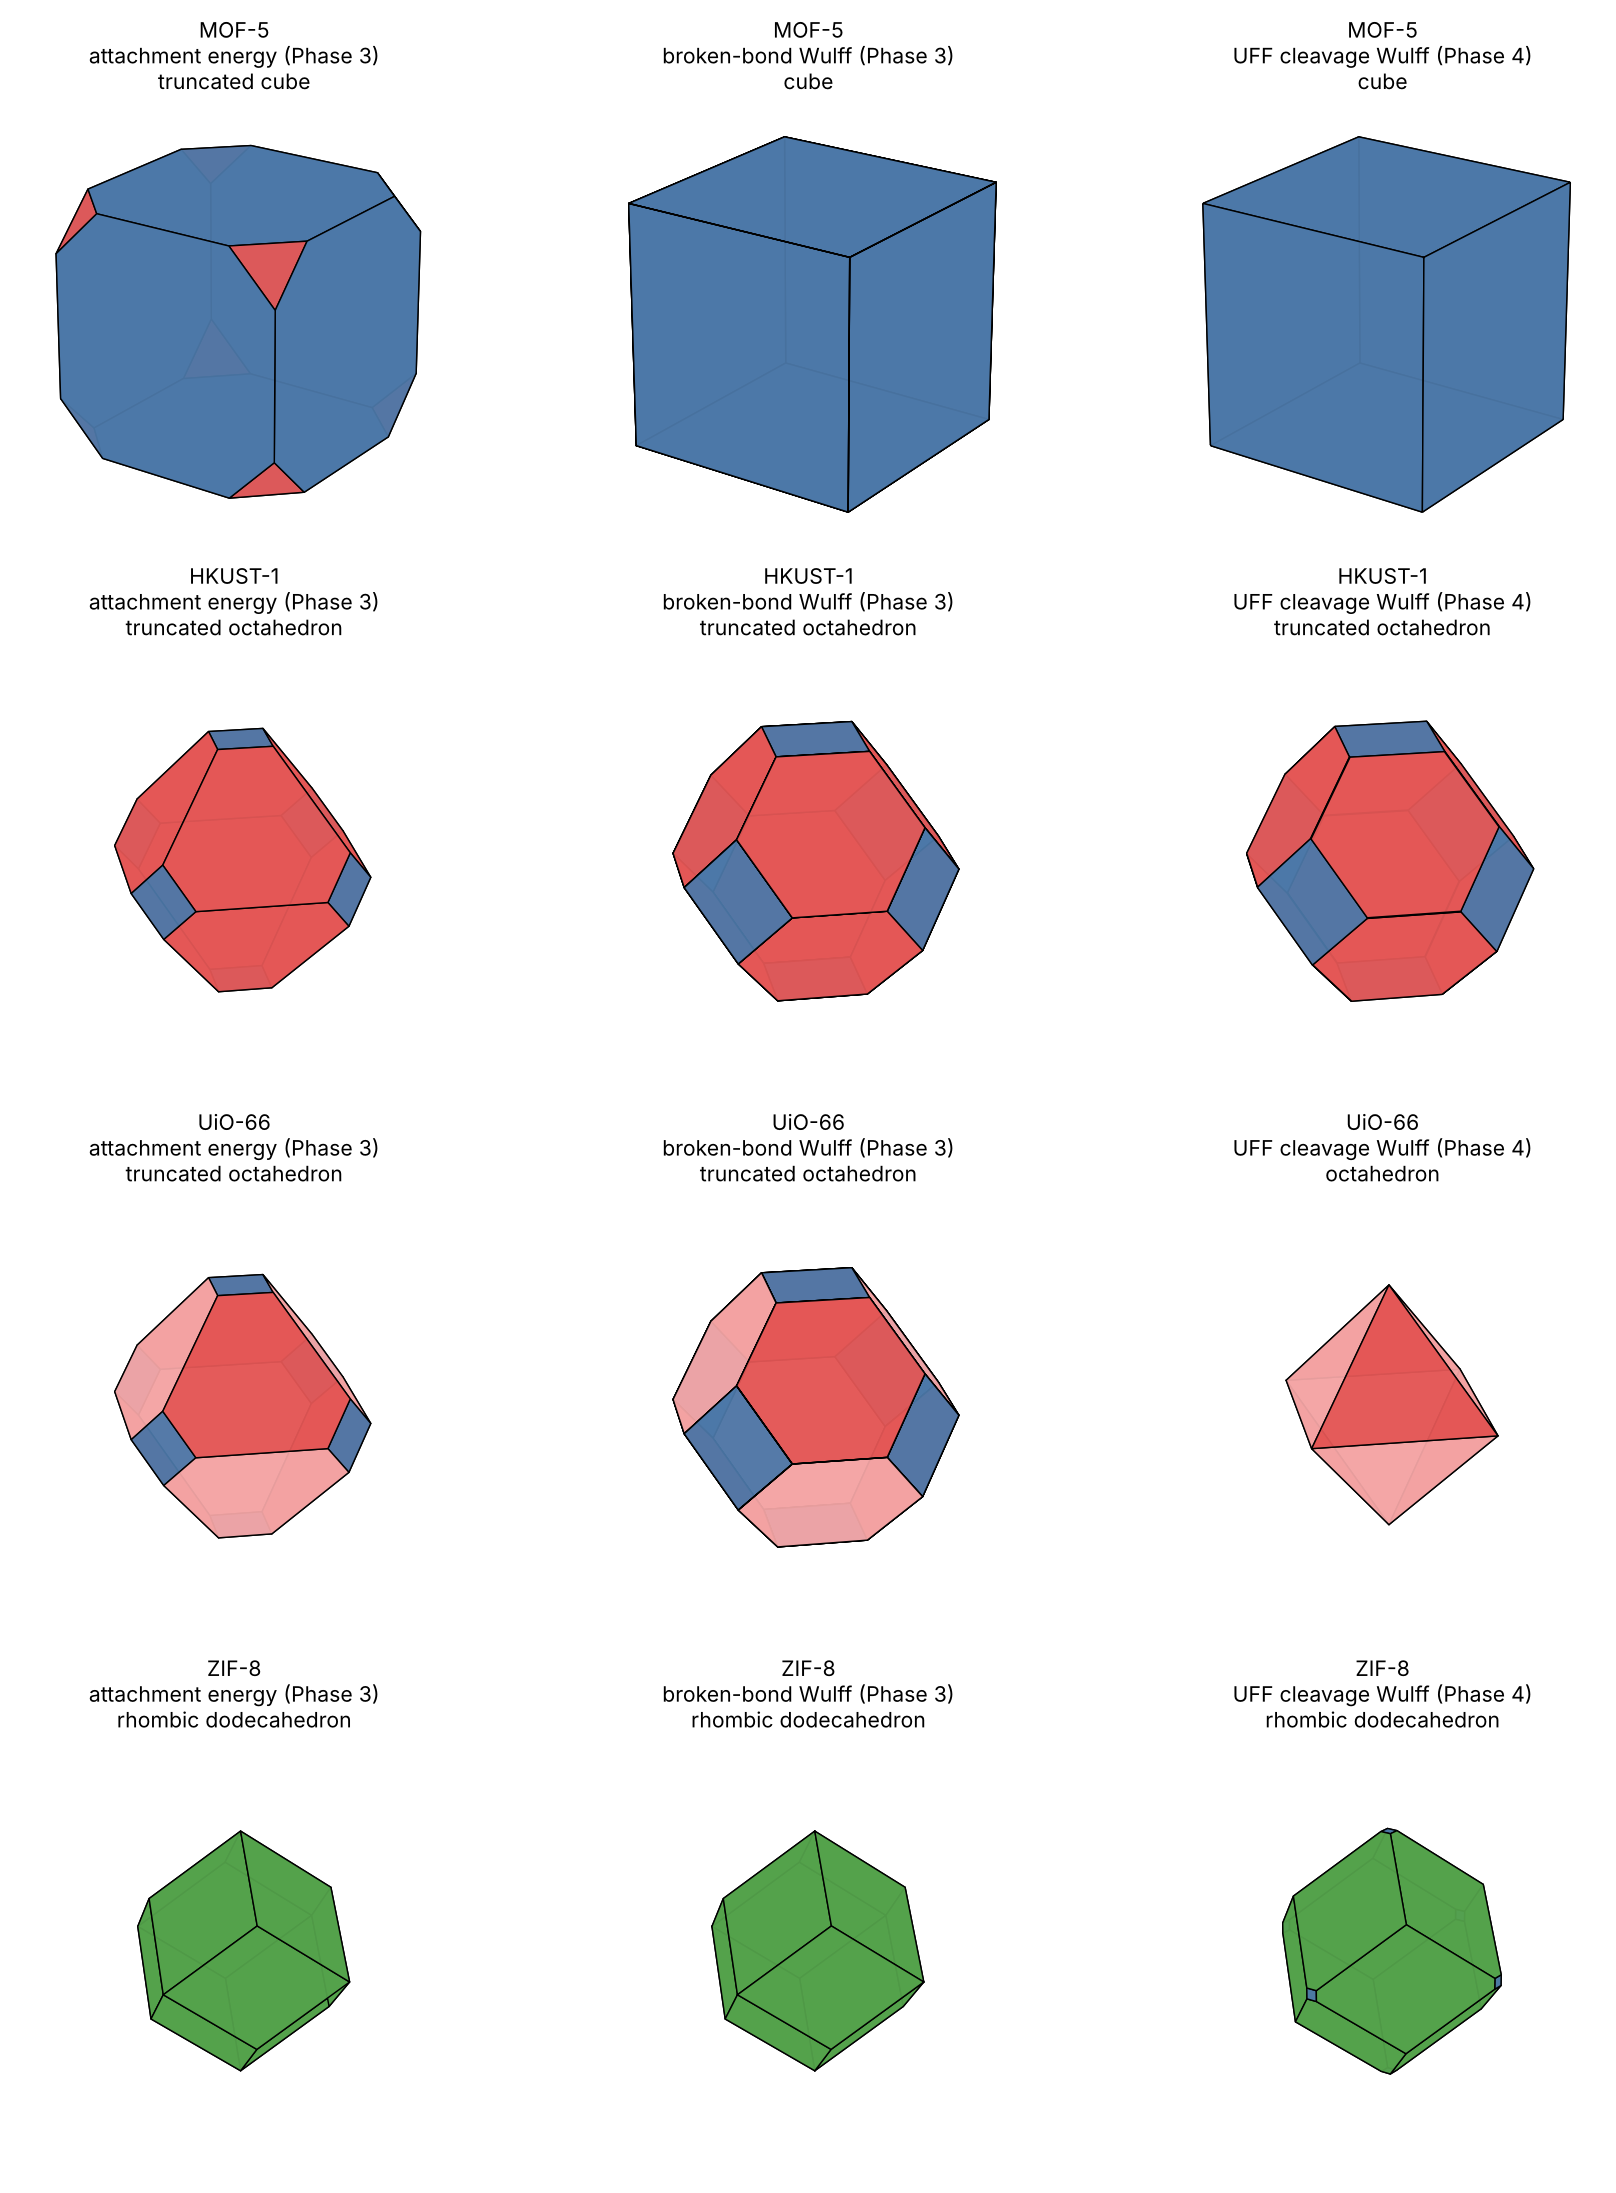
\includegraphics[width=0.48\textwidth]{figures/phase4_compare.png}\hfill
    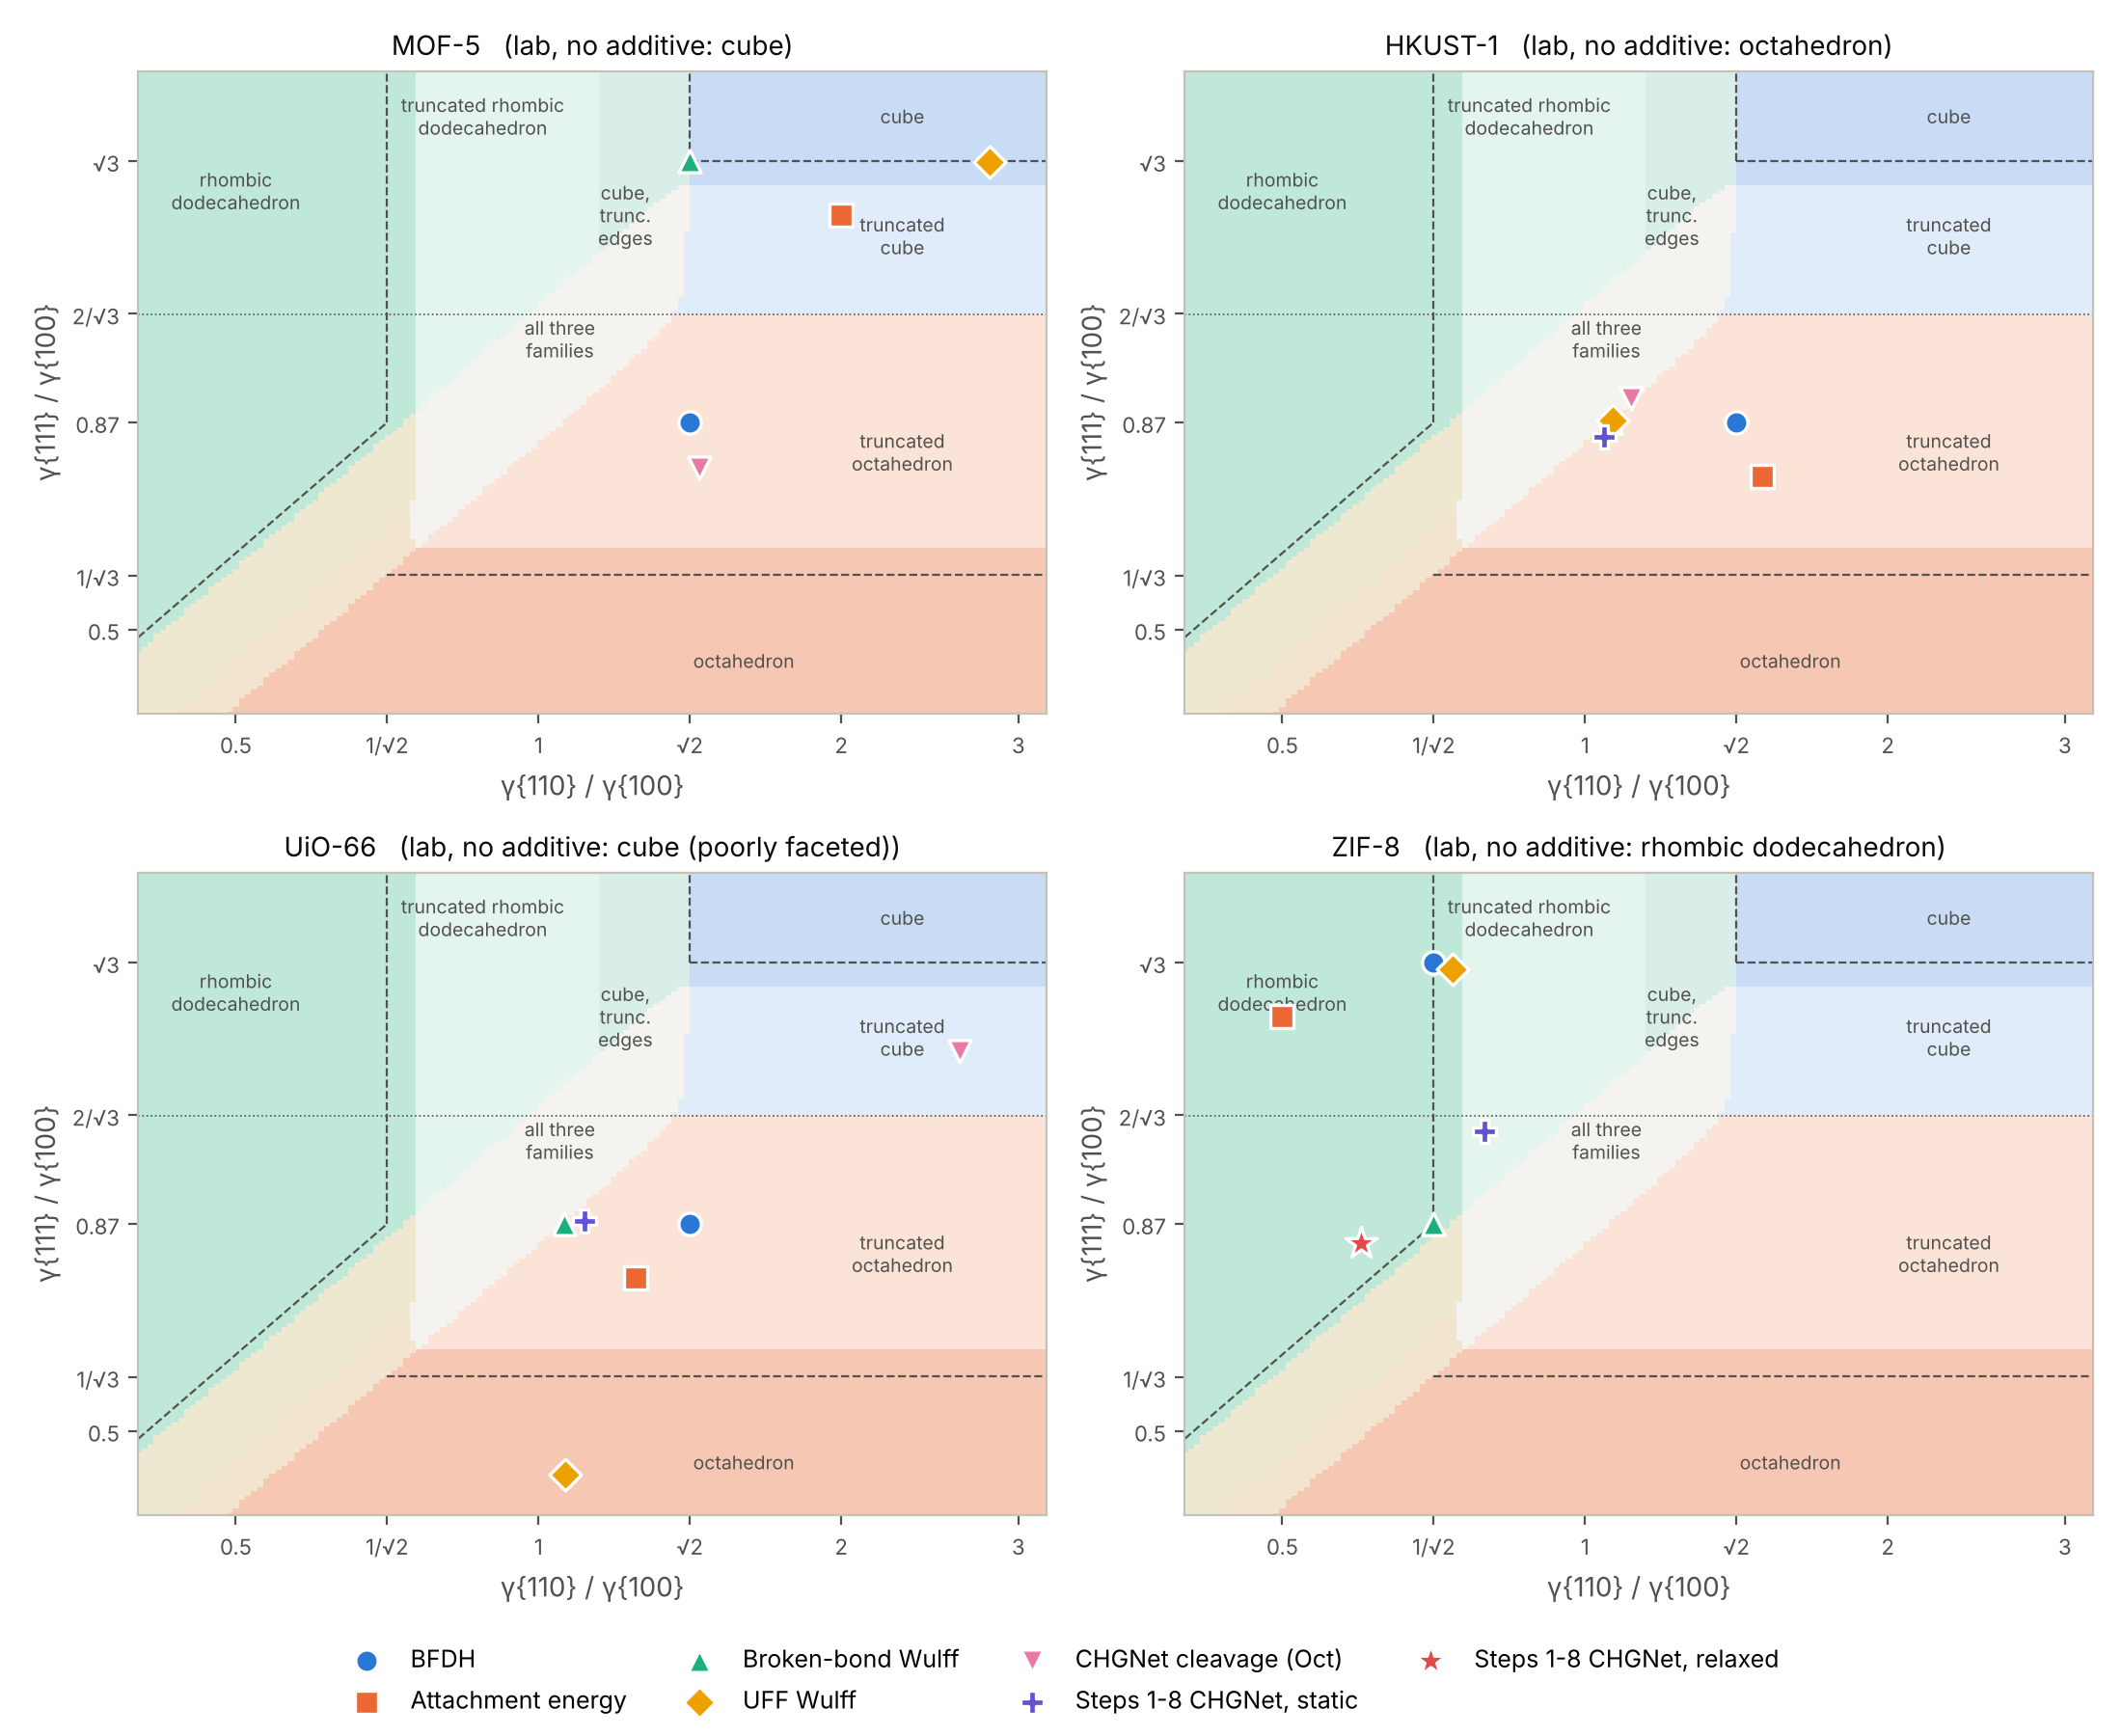
\includegraphics[width=0.48\textwidth]{figures/fig_map_models.png}
    \caption{Left: shapes of the four demonstration MOFs from three energy models (\texttt{figs\_phase4.py}). Right: each model as a point on the cubic morphology map (\texttt{morphology\_map/}). The Shape advisor page of the website shows the same for ten MOFs, in 3D, with steering and gas-access tables.}
\end{figure}
\noindent
\textbf{Discussion:} the structure-only model works where the crystal is grown without additives and the face order is set by strong bonds (MOF-5 cubes, ZIF-8 rhombic dodecahedra, HKUST-1 octahedral faces). It fails for UiO-66, whose additive-free crystals are poorly faceted cubes, and it cannot represent additives, which move different MOFs in different directions. MOF-5's ratio $\gamma_{111}/\gamma_{100} = 1.72$ lies 0.7\% below the cube boundary $\sqrt3$, so its ``cube'' rests on one constant.

\section{Technical Justification, Design Trade-offs \& Insights}
\begin{itemize}[noitemsep, topsep=2pt]
    \item \textbf{Why these models:} BFDH needs only symmetry and runs on any CIF; the bond-count energy adds what BFDH lacks with no fitting; DFT would be the reference but needs HPC time we do not have, and CHGNet, the fast alternative, is not validated for MOF surfaces. No learned model is trained: laboratory shapes exist for 12 MOFs, and learning from other MOFs gives 5 of 32.
    \item \textbf{Complexity:} absences and BFDH are $O(|G|\,h^3)$ for $|G|$ operations and index limit $h$; a cleavage curve is $O(P)$ for $P$ atom pairs within 12~\AA; a Wulff shape is a half-space intersection; everything runs in seconds per MOF.
    \item \textbf{Edge cases:} primitive cells are converted to the conventional cell; files stored in P1 or with ordered substituents (IRMOF-3, IRMOF-8, 71 of 77 hMOF files) have broken symmetry and are flagged; records without a dominant face are not scored for faces; three additive-free labels that are judgement calls are listed.
\end{itemize}

\section{Conclusion, Limitations \& Future Scope}
\begin{itemize}[noitemsep, topsep=2pt]
    \item \textbf{Conclusion:} from one unit cell the project generates the allowed faces, the family of shapes and the favoured shape of a MOF, mathematically and by program, and shows on 8 MOFs and 134 records that the structure alone gives the dominant face of additive-free crystals for 4 of 5 MOFs.
    \item \textbf{Limitations:} unrelaxed energies without electrostatics or solvent; only MOF-5 separates the energy models; no model predicts additives; gas access is geometric (an open point may not connect to the pore network), not adsorption; one person extracted the laboratory records and checked the proofs.
    \item \textbf{Future scope:} DFT on six prepared slabs (MOF-5, UiO-66, HKUST-1); a relaxed CHGNet run with the steps 1--8 fixes; additive binding energies per face; pore-network accessibility (Zeo++); a blind second extraction of 20 laboratory records.
\end{itemize}

\section{Project Deliverables \& Technical Enrichment Summary}
\begin{table}[H]
    \centering
    \footnotesize
    \renewcommand{\arraystretch}{1.15}
    \begin{tabular}{|p{4.0cm}|p{9.2cm}|c|}
        \hline
        \textbf{Deliverable} & \textbf{Details} & \textbf{Status} \\
        \hline
        Source code repository & \url{https://github.com/Radha-Krishna-19/fyp}: code, data, tests, CI, READMEs & Completed \\
        \hline
        Online certifications & Fractals and Scaling; Introduction to Complexity (Santa Fe Institute); Graph Theory; Graph Algorithms in Java and Social Network Analysis (Udemy); Graph Algorithms for Machine Learning (TigerGraph) & Completed \\
        \hline
        Group activity: website & Documentation portal, 27 pages, two engines, tests & Completed \\
        \hline
        Group activity: dataset release & Spectrum descriptors (CC BY 4.0) and the 134-record morphology dataset & Completed \\
        \hline
        Group activity: research paper & Team paper on the coarse-grained spectrum (\texttt{docs/paper/}) & Draft submitted \\
        \hline
    \end{tabular}
    \caption{Project and technical enrichment deliverables.}
\end{table}

\vspace{0.1cm}
\nocite{*}
\renewcommand{\refname}{\large\bfseries\color{amritaMaroon}References}
\bibliographystyle{ieeetr}
{\footnotesize \bibliography{ref}}

\end{document}
